

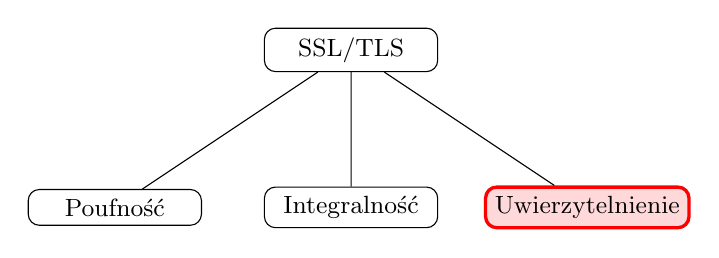
\begin{tikzpicture}[
		level distance=20mm,
		sibling distance=30mm,
		every node/.style={
				draw,
				rounded corners,
				align=center,
				minimum width=22mm,
				font=\small
			},
		highlight/.style={
				draw=red,
				very thick,
				fill=red!15
			}
	]
	\node {SSL/TLS}
	child { node {Poufność} }
	child { node {Integralność} }
	child { node[highlight] {Uwierzytelnienie} };
\end{tikzpicture}
